\section{Experiments}
\label{chap:experiments }

The data-set \cite{pipattanasomporn2020cu} comes from smart high-rise building in Thailand with 1.5 years of data collected at 1 minute resolution. 
We investigate 24 zones equipped with ambient sensors and power consumption meter.  
The analysis is presented in three parts : a) evaluate the accuracy of the virtual field with all sensors, b) understand the effect of removing sensors by comparing our algorithm with a baseline for the optimal sensor placement problem c) understanding trade-offs in a multi objective optimization.  

\subsection{Virtualization Accuracy}

\begin{figure}
    \centering
    \subfloat[ $M^z$ where z = Floor 7 Zone 5 ]{{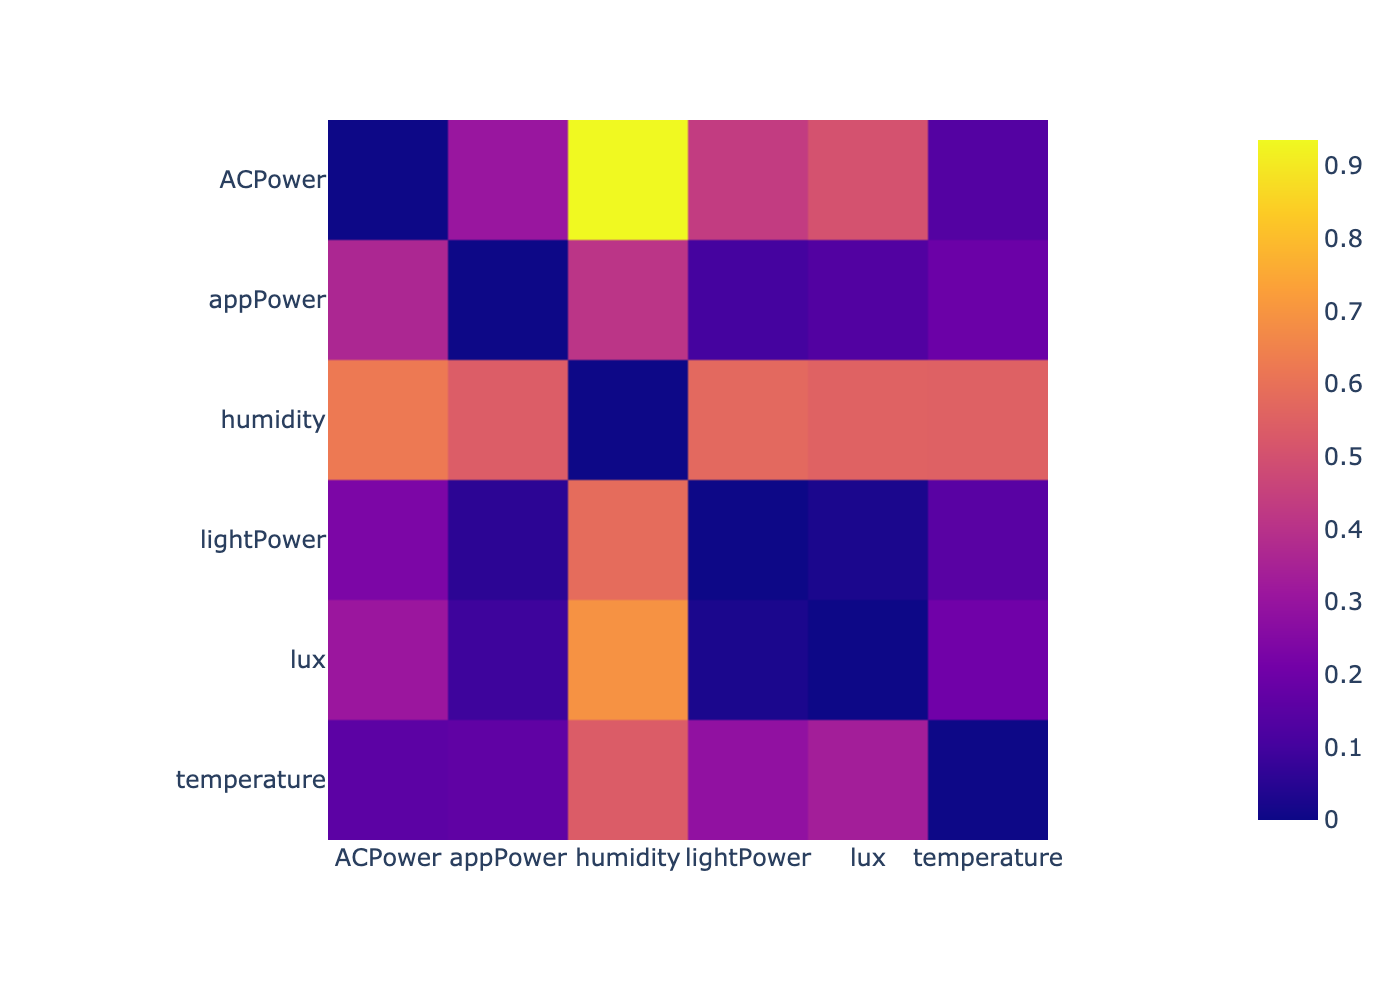
\includegraphics[width=0.47\textwidth]{img/4567fzone/Floor4Z1.png} }}%
    \qquad
    \subfloat[\centering $M^z$ where z =  Floor 4 Zone 1] {{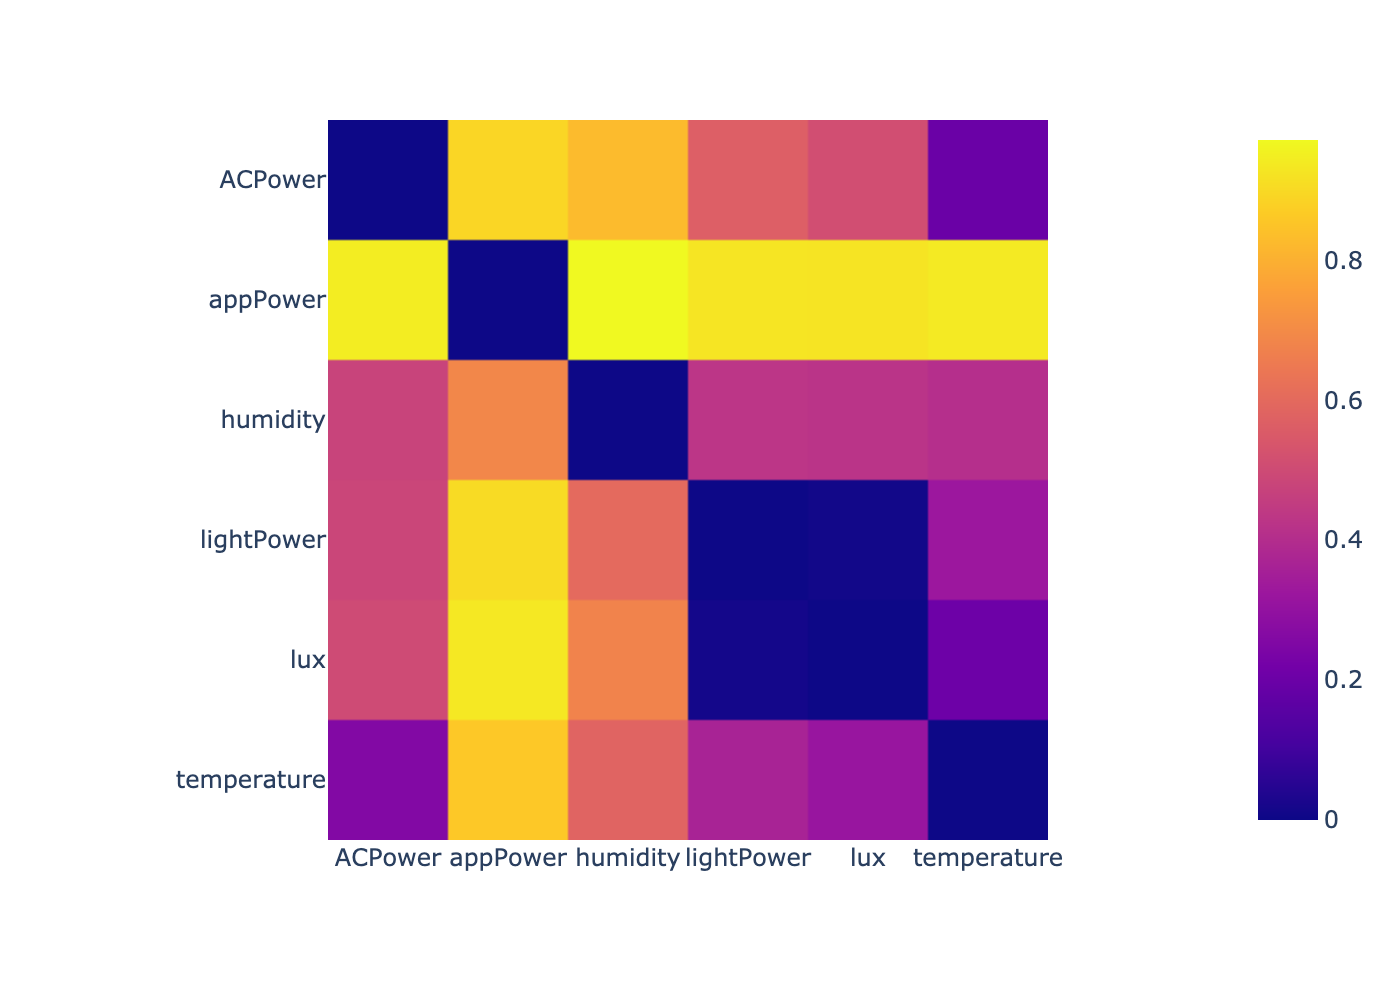
\includegraphics [width=0.47\textwidth] {img/4567fzone/Floor7Z5.png} }}%
    \caption{Error Matrix for 2 zones}
    \label{fig:zoneVirtualize}%
\end{figure}

To guess a sensor $v \in A^c(g)$, the system learn a set of supervised machine learnt predictors with a single channel data input $u \in A^c(g), u \neq v$.
For every group, $O(|A^c(g)|^2)$ learners are trained to capture the intra group sensor dynamics. 
For a prediction task, a learner picks the least erred model from a set of classical algorithms:  linear regression, lasso net, random forest, and XGBoost.
Let for a group $g$ the approximated ($A_g$) and ground truth are represented by vectors $\hat{y}^z_s$ and $y^z_s$ for sensor $s$ at location $z$ respectively. 
The mean squared error is given as
\begin{equation*}
L_{MSE} =\frac{1}{KZ}\sum_{k \in K} \sum_{z \in Z} (\hat{y}^z_s - y^z_s)^2 
\end{equation*}
%  show the effect of vertical orientation on the virtualization accuracy for 2 zones. 
First we check the effect of spatial grouping on the virtual sensor field accuracy.
% We see that appliance power (MSE $\approx 0.9$) is the worst approximation on Floor 4 Zone 1 (F4 Z1), while it is humidity (MSE $\approx 0.8$)  for Floor 7 (F7 Z5).
Variations in Figure \ref{fig:zoneVirtualize} is explained by the fact that zone 5 is from top Floor 7 and experiences a harsher environment like direct sun light, higher temperature/humidity fluctuations than zone 1 of Floor 4.
Figures \ref{fig:domainVirtualizeAmbience} and \ref{fig:domainVirtualizePower} show the  virtualization error for domain wise grouping as a heat-map covering all zones.
 We observe that AC Power bears a negative correlation with temperature and humidity when AC is turned on primarily for cooling.
Light Power is positively related to indoor luminosity levels by observing at night the lights are off and during day, the lights are turned on for acceptable visibility levels.
Power consumed due to appliances has an inverse affinity for temperature and humidity, which likely indicate working conditions in a controlled thermal environment.
% Temperature and humidity also has a negative correlation with AC and appliance power intuitively meaning appliances are running more when ambience is controlled due to occupancy.
% Figure \ref{fig:ambient2acpower} shows the prediction of light power from luminosity and AC Power from temperature. 

\begin{table}[]
\begin{tabular}{|l|l|l|l|l|l|l|}
\hline
Zone & \multicolumn{3}{l|}{Power} & \multicolumn{3}{l|}{Ambience} \\ \hline
 &   AC  & Light   & App     & Temp     & RH    & Lux             \\ \hline
Floor2Z1 & 0.15                         & 0.14                            & 0.13                          & \textbf{0.18    }                         & 0.53                          & 0.15                     \\ \hline
Floor2Z2 & \textbf{0.08   }                      & 0.07                            & 0.15                          & \textbf{0.11    }                       & 0.36                          & \textbf{0.06     }                \\ \hline
Floor2Z4 & 0.33                         & 0.31                            & 0.73                          & 0.33                             & 0.66                          & 0.31                     \\ \hline
Floor3Z1 & 0.32                         & 0.23                            & 0.38                          & 0.24                             & 0.45                          & 0.26                     \\ \hline
Floor3Z2 & 0.35                         & 0.25                            & 0.27                          & 0.29                             & 0.4                           & 0.27                     \\ \hline
Floor3Z4 & 0.34                         & 0.23                            & 0.25                          & 0.22                             & 0.61                          & 0.22                     \\ \hline
Floor3Z5 & 0.42                         & 0.25                            & 0.27                          & 0.28                             & 0.63                          & 0.24                     \\ \hline
Floor4Z1 & 0.28                         & 0.24                            & 0.19                          & 0.2                              & 0.53                          & 0.26                     \\ \hline
Floor4Z2 & 0.34                         & 0.27                            & 0.48                          & 0.25                             & 0.59                          & 0.25                     \\ \hline
Floor4Z4 & 0.28                         & 0.25                            & 0.29                          & 0.24                             & 0.53                          & 0.24                     \\ \hline
Floor4Z5 & 0.36                         & 0.18                            & 0.35                          & 0.23                             & 0.46                          & 0.17                     \\ \hline
Floor5Z1 & 0.23                         & 0.2                             & 0.19                          & 0.15                             & 0.45                          & 0.22                     \\ \hline
Floor5Z2 & 0.29                         & 0.19                            & 0.28                          & 0.19                             & 0.35                          & 0.19                     \\ \hline
Floor5Z4 & 0.33                         & 0.36                            & 0.31                          & 0.3                              & 0.58                          & 0.3                      \\ \hline
Floor5Z5 & 0.43                         & 0.26                            & 0.29                          & 0.31                             & 0.64                          & 0.26                     \\ \hline
Floor6Z1 & 0.26                         & 0.23                            & 0.25                          & 0.29                             & 0.37                          & 0.22                     \\ \hline
Floor6Z2 & 0.36                         & 0.28                            & 0.22                          & 0.28                             & 0.38                          & \textbf{0.3  }                    \\ \hline
Floor6Z4 & 0.26                         & 0.17                            & 0.27                          & 0.22                             & 0.41                          & 0.21                     \\ \hline
Floor6Z5 & 0.47                         & 0.22                            & 0.26                          & 0.23                             & 0.58                          & 0.23                     \\ \hline
Floor7Z1 & 0.34                         & 0.28                            & 0.43                          & 0.31                             & 0.65                          & 0.48                     \\ \hline
Floor7Z2 & 0.31                         & 0.3                             & 0.59                          & 0.33                             & 0.61                          & 0.23                     \\ \hline
Floor7Z4 & 0.28                         & 0.21                            & 0.28                          & 0.23                             & 0.41                          & 0.2                      \\ \hline
Floor7Z5 & 0.44                         & 0.38                            & 0.71                          & 0.34                             & \textbf{0.61  }                        & 0.36                     \\ \hline

\end{tabular}
\caption{Virtual Sensor Field Accuracy ($L_s$) with Spatial Grouping or predicting a cell using \textbf{columns from the same row}.}
\label{table:vsfAccuracySpatial}
\end{table}

\begin{table}[]
\begin{tabular}{|l|l|l|l|l|l|l|}
\hline
Zone & \multicolumn{3}{l|}{Power} & \multicolumn{3}{l|}{Ambience} \\ \hline
 &   AC  & Light   & App     & Temp     & RH    & Lux             \\ \hline
Floor2Z1 & 0.08                     & 0.07                             & 0.11                          & 0.25                         & 0.14                          & 0.05                            \\ \hline
Floor2Z2 & 0.09                     & 0.06                             & 0.13                          & 0.24                         & 0.25                          & 0.09                            \\ \hline
Floor2Z4 & 0.09                     & 0.06                             & 0.12                          & 0.26                         & 0.66                          & 0.06                         \\ \hline
Floor3Z1 & 0.11                     & 0.03                             & 0.08                          & 0.04                         & 0.26                          & 0.03                            \\ \hline
Floor3Z2 & 0.07                     & 0.04                             & 0.09                          & 0.05                         & 0.17                          & 0.03                            \\ \hline
Floor3Z4 & 0.09                     & 0.03                             & 0.11                          & 0.06                         & 0.23                          & 0.03                            \\ \hline
Floor3Z5 & 0.08                     & 0.03                             & 0.1                           & 0.07                         & 0.18                          & 0.05                            \\ \hline
Floor4Z1 & 0.08                     & 0.03                             & 0.08                          & 0.06                         & 0.16                          & 0.05                            \\ \hline
Floor4Z2 & 0.06                     & 0.02                             & 0.11                          & 0.05                         & 0.44                          & 0.04                            \\ \hline
Floor4Z4 & 0.07                     & 0.02                             & 0.08                          & 0.05                         & 0.22                          & 0.05                            \\ \hline
Floor4Z5 & 0.14                     & 0.03                             & 0.08                          & 0.07                         & 0.36                          & 0.06                            \\ \hline
Floor5Z1 & 0.15                     & 0.03                             & 0.13                          & 0.06                         & 0.2                           & 0.08                            \\ \hline
Floor5Z2 & 0.08                     & 0.03                             & 0.09                          & 0.07                         & 0.29                          & 0.04                            \\ \hline
Floor5Z4 & 0.17                     & 0.03                             & 0.09                          & 0.06                         & 0.17                          & 0.04                            \\ \hline
Floor5Z5 & 0.07                     & 0.05                             & 0.12                          & 0.05                         & 0.13                          & 0.04                            \\ \hline
Floor6Z1 & 0.12                     & 0.04                             & 0.08                          & 0.04                         & 0.25                          & 0.13                            \\ \hline
Floor6Z2 & 0.27                     & 0.03                             & 0.08                          & 0.06                         & 0.19                          & 0.32                            \\ \hline
Floor6Z4 & 0.14                     & 0.04                             & 0.1                           & 0.06                         & 0.26                          & 0.09                            \\ \hline
Floor6Z5 & 0.1                      & 0.04                             & 0.09                          & 0.12                         & 0.3                           & 0.09                            \\ \hline
Floor7Z1 & 0.64                     & 0.05                             & 0.12                          & 0.08                         & 0.36                          & 0.08                            \\ \hline
Floor7Z2 & 0.08                     & 0.05                             & 0.08                          & 0.09                         & 0.5                           & 0.14                            \\ \hline
Floor7Z4 & 0.07                     & 0.03                             & 0.09                          & 0.08                         & 0.35                          & 0.03                            \\ \hline
Floor7Z5 & 0.08                     & 0.03                             & 0.08                          & 0.09                         & 0.63                          & 0.05                            \\ \hline

\end{tabular}
\caption{Virtual Sensor Field Accuracy ($L_d$) with Domain Wise Grouping or predicting a cell using \textbf{rows from the same column}.}
\label{table:vsfAccuracyDomain}
\end{table}

\begin{equation}\begin{matrix}
L_s [z,d] = & \Sigma_{v \in A^c(g=z)} \frac{M^z[v,d]}{|A^c(g=z)|}  \\
L_d [z,d] = & \Sigma_{v \in A^c(g=d)} \frac{M^d[v,z]}{|A^c(g=d)|} 
\end{matrix}
\end{equation}
Due to lack to space, it is impossible to show all $M^g$ tables, instead we report the spatial ($L_s$) and domain ($L_d$) wise loss to fill up Table \ref{table:vsfAccuracySpatial} and \ref{table:vsfAccuracyDomain} respectively.
% Apart from zone 1, zone 2 of Floor 2 and zone 5 of floor 7,
Amongst all the sensors, relative humidity is most difficult to approximate,  $L_s$ (min=0.37, max=0.66) and $L_d$ = (min=0.14, max=0.63)  across all zones.
Amongst the ambient sensors, luminosity (lux) levels has the best $L_d$  (min=0.03, max=0.14) although for Floor 2 Zone 2, we observe $L_s=0.06 > L_d = 0.09$.  
For, indoor temperature prediction $L_d$  (min=0.04, max=0.14)  is lower than $L_s$ (min=0.19, max=0.71) for all floors except in floor 2 with zone 1 $L_s = 0.18, L_d=0.25$ and zone 2 $L_s = 0.11, L_d = 0.24 $.
Power Consumption pattern is usually continuous but "non-differentiable" in nature arising due to sharp peaks and crests for fast response times.  
The ability to learn the patterns from inter zonal power consumption $L_d =$ (min= 0.03, max=0.27)  is more effective rather using intra-zonal data sources  $L_s =$ (min= 0.2, max=0.71)   for predicting light, AC, and appliance channels.
Majorly, we see that domain wise grouping performs better on average which confirms the intuitiveness of being guessed \textit{easily} by similar peers.
For every type of sensor, the error matrix for ambient and power consumption sensors are visualised as a heat-map in Figures \textbf{\ref{fig:domainVirtualizeAmbience} and \ref{fig:domainVirtualizePower}} respectively.

 
\subsection{ Baseline Comparison }

We compare our approach with a similar type of problem that eliminates non redundant ones from a sensor set.
For a fair comparison, we evaluate the value of the objective set $O = [O^v_b, O^v_f]$ at every solution point.
The baseline algorithm starts with a signal decomposition step where instantaneous phase estimates (IP), instantaneous frequency estimates (IF), and instantaneous amplitude estimates (IA) are extracted per sensor.
Unsupervised learning is applied to the Intrinsic Mode Function space spanned by (IP,IF,IA) to generate clusters.
The parameter space for K-Means \cite{likas2003global} is varied between $k \in [30, 90]$ and for DBSCAN \cite{schubert2017dbscan} the range for minimum clubbing distance "\textit{eps}" $\in [ 0.01,0.04 ] $ and minimum number of samples $\in [6,23]$. 
For every cluster, we take $q$ candidate points and encode them as $\{0,1\}$ and take the minimum $[O^v_b, O^v_f]$ obtained from spatially and domain wise encoding.
Figure \ref{fig:baselineSupport} shows the scatter plot between forward and backward translation errors for the baseline algorithms and our approach.
The dual objective values from  K-Means and DBSCAN converge to an error region of ($O^v_f, O^v_b \in [0.3-0.5]$) while the best solution yielded by evolutionary computing has ($O^v_f, O^v_b \in [0.20-0.25]$). 
In contrast to unsupervised learning, our algorithm generates a Pareto front as per Figure Fig \ref{fig:baselineSupport} where no objective can decrease without increasing another.
From Figure \ref{fig:tradeoffForwardBackward}, we observe that using $[60,85]$ sensors, the forward translation MSE $ \in [0.05, 0.1]$ with a backward margin between $[0.2,0.25]$ .
Out of 138 sensors, the system achieves a fair trade-off between forward and backward translation MSE [0.16, 0.19] with approximately $45-50 \%$ less sensors. 
Increasing number of observable sensors, decreases $O^v_f$ to MSE [0.05] using 80-85 sensors while the backward error $O^v_b$ increases to 0.48 since more number of difficult sensor patterns have to be approximated now.




\begin{figure}%
    \centering
    \subfloat[ Baseline Comparison  ]{{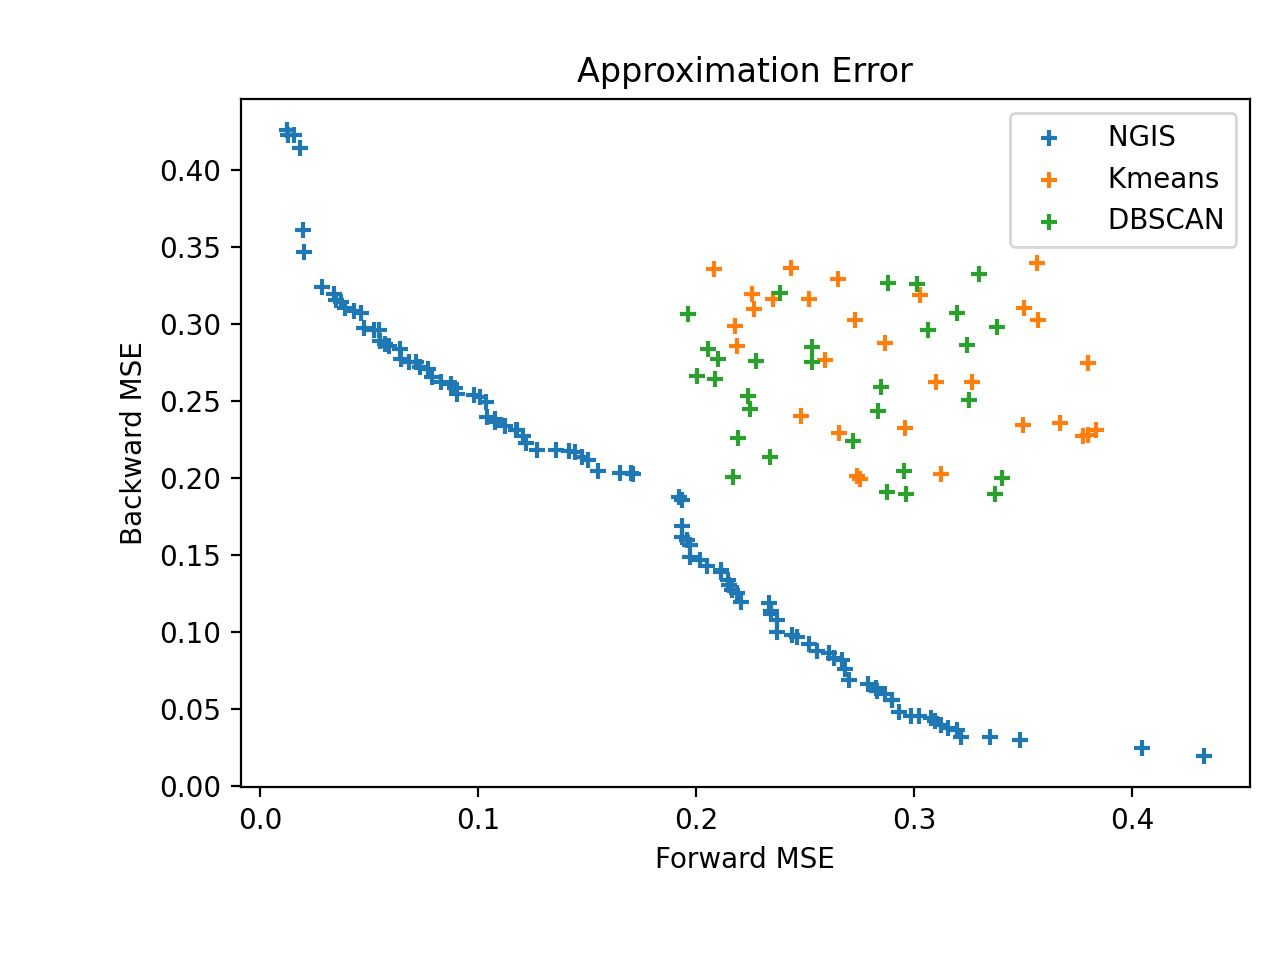
\includegraphics[width=0.47\textwidth]{img/baselineComp.png} }\label{fig:baselineSupport}}%
    \qquad
    \subfloat[\centering Dual Objective Optimization] {{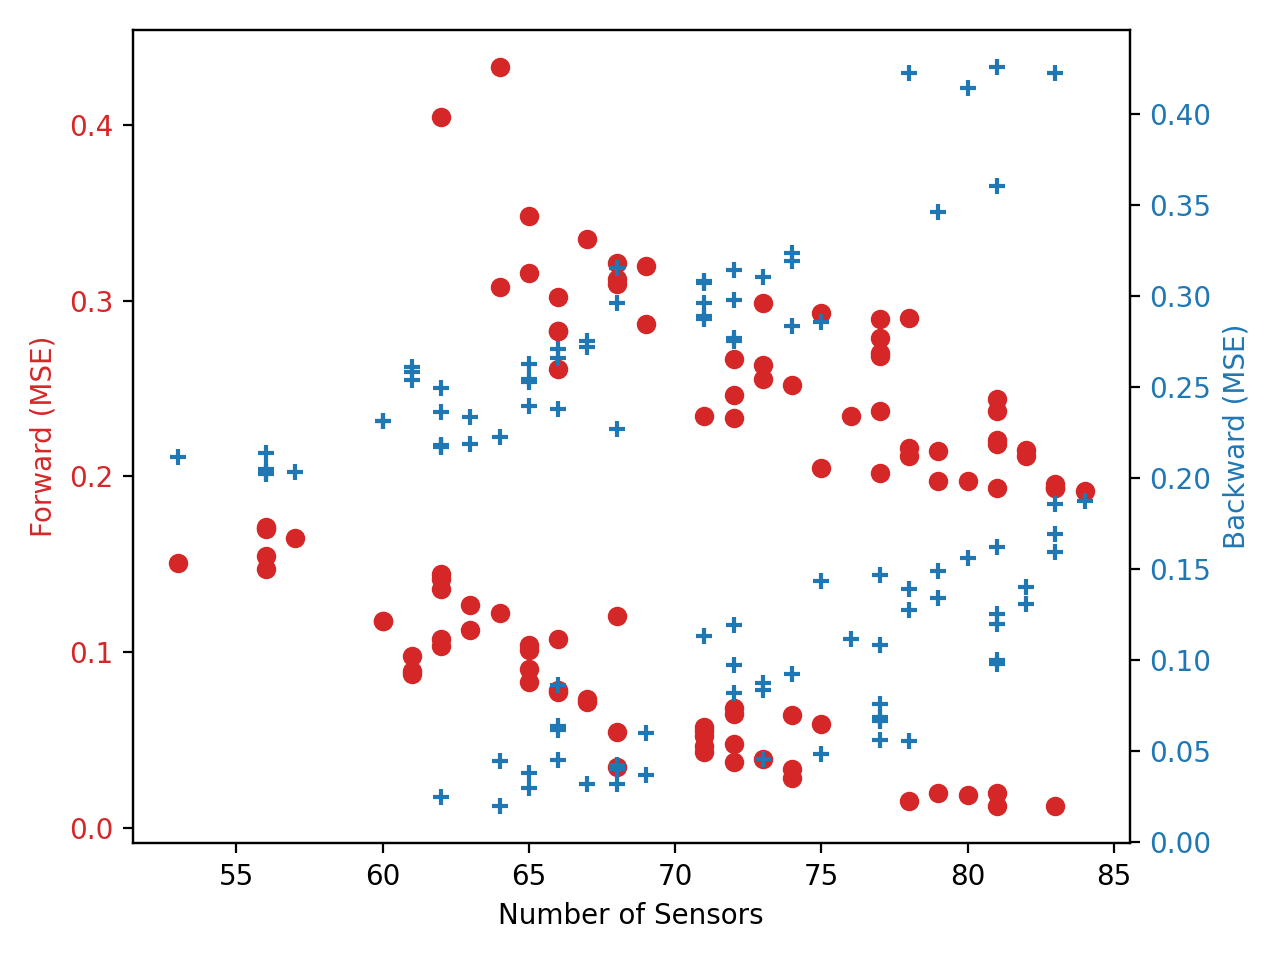
\includegraphics [width=0.47\textwidth]{img/tradeoffForwardBackward.png} }\label{fig:tradeoffForwardBackward}}%
    \caption{ Algorithm Performance Comparison on bidirectional losses while approximating between Support and Approximated Sets.}
    \label{fig:baselineComp}%
\end{figure}


\subsection{Segmented Business Trade-offs }


\begin{figure}%
    \centering
    \subfloat[ Forward Accuracy ]{{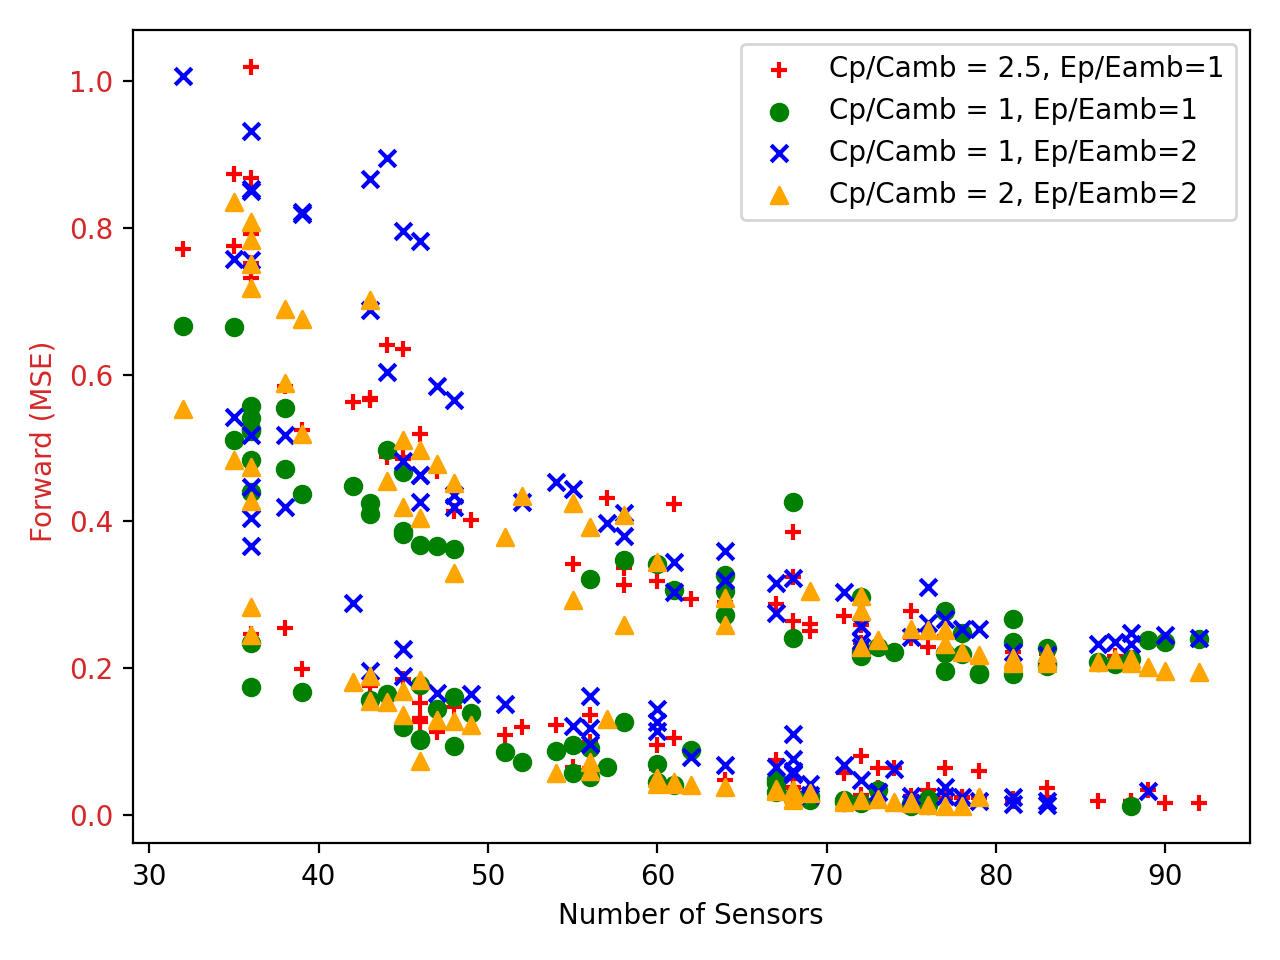
\includegraphics[width=0.47\textwidth]{img/forwardVar.png} }\label{fig:forwardVar}}%
    \qquad
    \subfloat[\centering Backward Translation Error] {{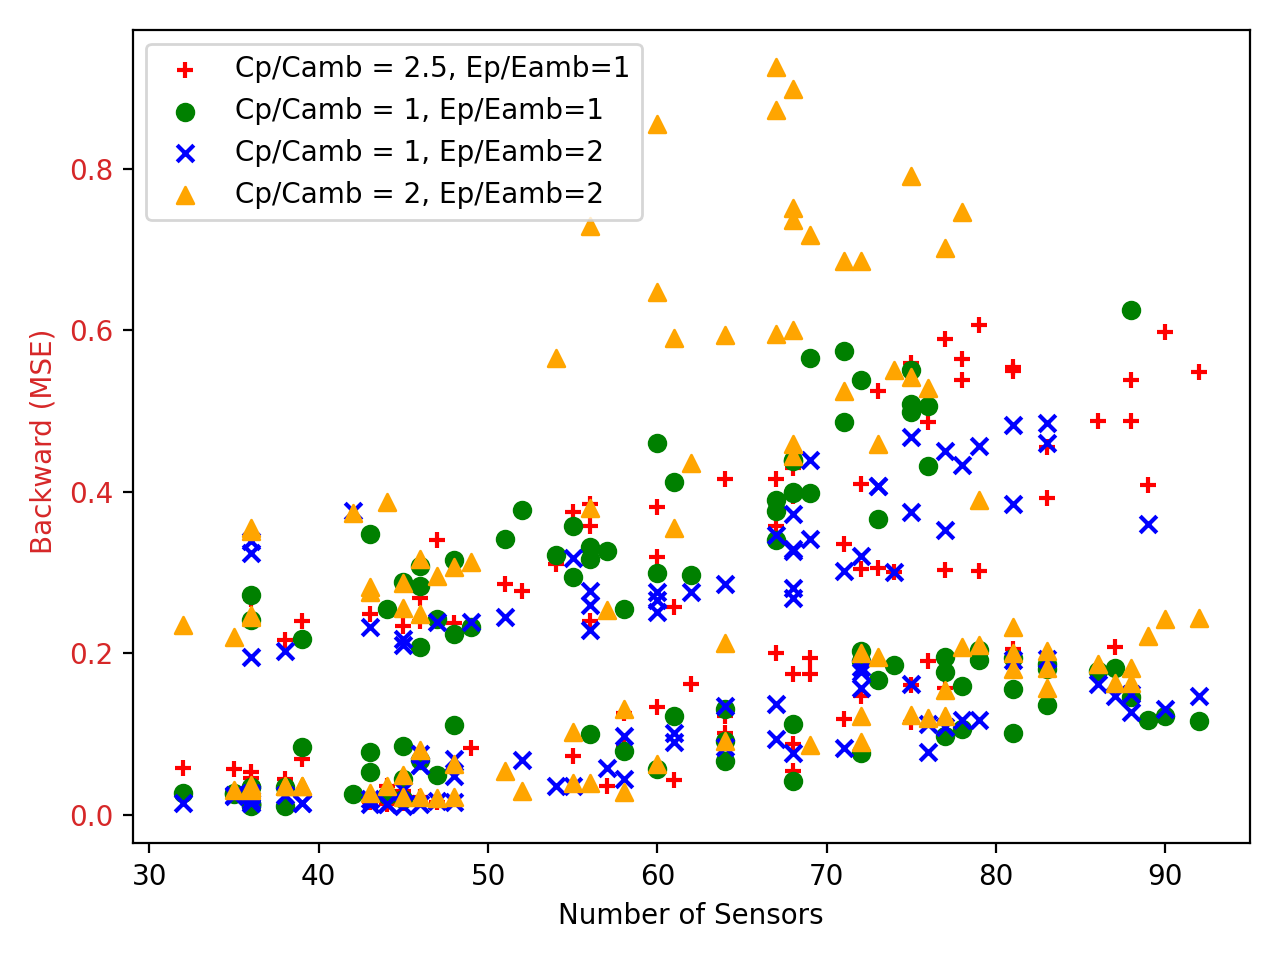
\includegraphics [width=0.47\textwidth]{img/backwardVar.png} }\label{fig:backwardVar}}%
    \caption{Backward Translation Error of last generation candidates in the Building Chromosome Gene Pool.}
    \label{fig:fwdbkwdVar}%
\end{figure}

\begin{table}[]
\begin{tabular}{|l|l|l|}
\hline
      Market Segments           & Ambiencer  (QoS)    & Power (QoS)      \\ \hline
Home Solutions   &  DIY  &  DIY  \\ \hline
Co Working Zones & Industrial & DIY \\ \hline
Community Spaces & DIY & Industrial \\ \hline
Commercial & Industrial & Industrial \\ \hline
\end{tabular}
\caption{Classification of Market Segmentation with hardware requirement types for monitoring.}
\label{table:marketSegment}
\end{table}


We now study the effect of grouping with respect to the virtualization accuracy, monitory risk and energy foot-printing.
Average cost is around $[10-20] \$$ for ambient sensors like humidity, temperature while smart meters can be expensive around $[50-100] \$$.
We observe that the industrial or DIY embedded sensor hardware are typically between $[10-25]$ Watts.
Assuming 30 days a month, a 5W sensor will consume close to $5\times 24 \times 30 = 3.6 $ energy units (kWh) monthly. 
Industrial grade quality of smart sensor or power consumption meters can be more energy efficient but expensive than assembled Do-It-Yourself counterparts. 
Let the cost and energy consumption ratio between power meters and ambient sensor is given by $\frac{C_p}{C_{amb}} = \frac{P^r_{g\neq Amb}}{P^r_{g=Amb}}$ and $\frac{E_p}{E_{amb}} = \frac{P^w_{g\neq Amb}}{P^w_{g=Amb}}$.
We meet the requirements of Table \ref{table:marketSegment} through $2 \times 2$ factorial design with $\frac{C_p}{C_{amb}} \in \{1,2.5\}$ and $\frac{E_p}{E_{amb}} \in \{1,2\}$.
% to test the effect of hardware quality and annual energy footprint on power and ambient sensors.

\begin{figure}%
    \centering
    \subfloat[ Approximation of Bill of Materials  ]{{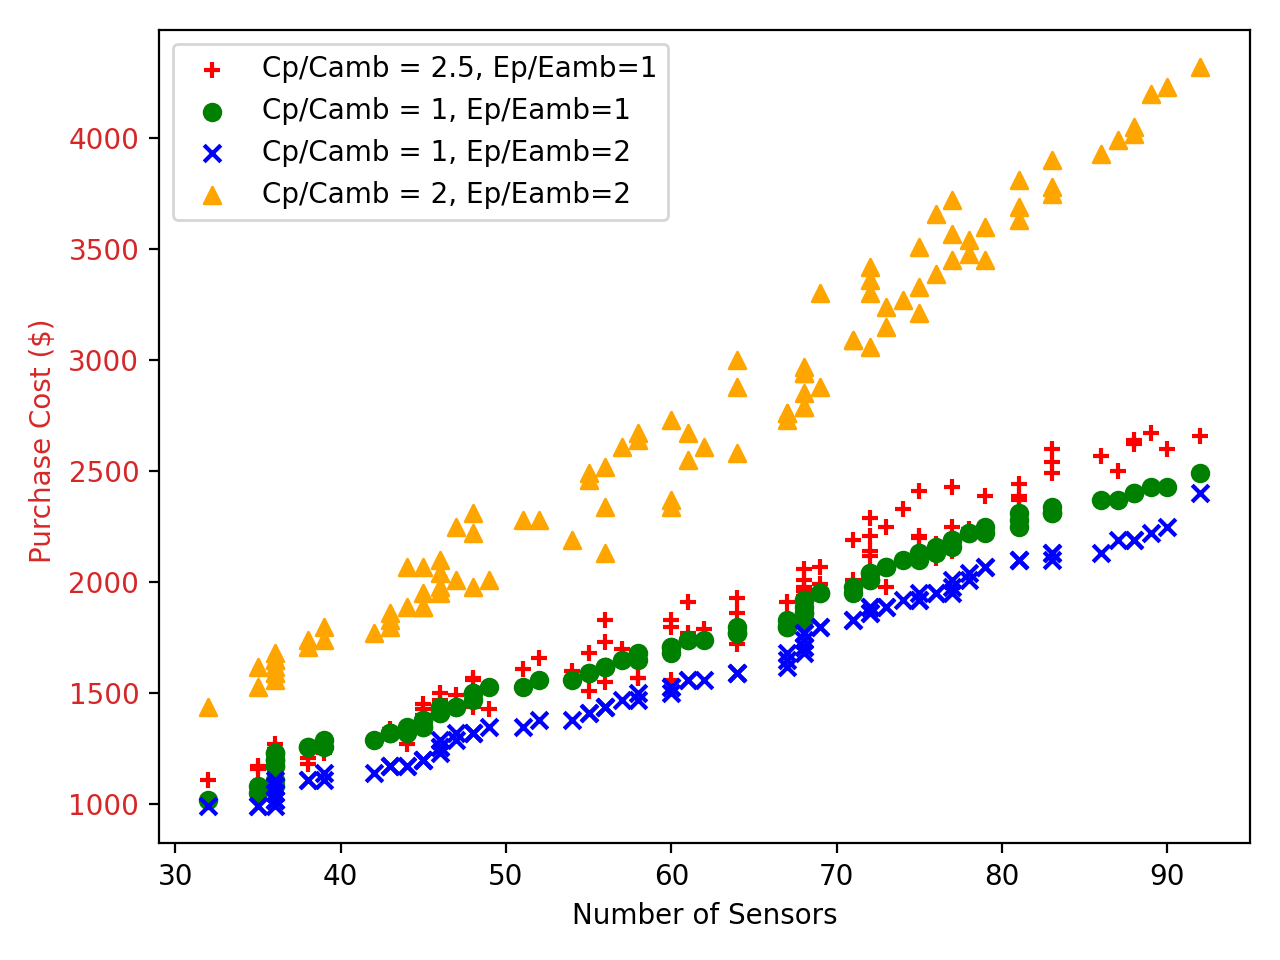
\includegraphics[width=0.47\textwidth]{img/installCostVar.png} }\label{fig:installCostVar}}%
    \qquad
    \subfloat[\centering Optimizing Energy Footprint] {{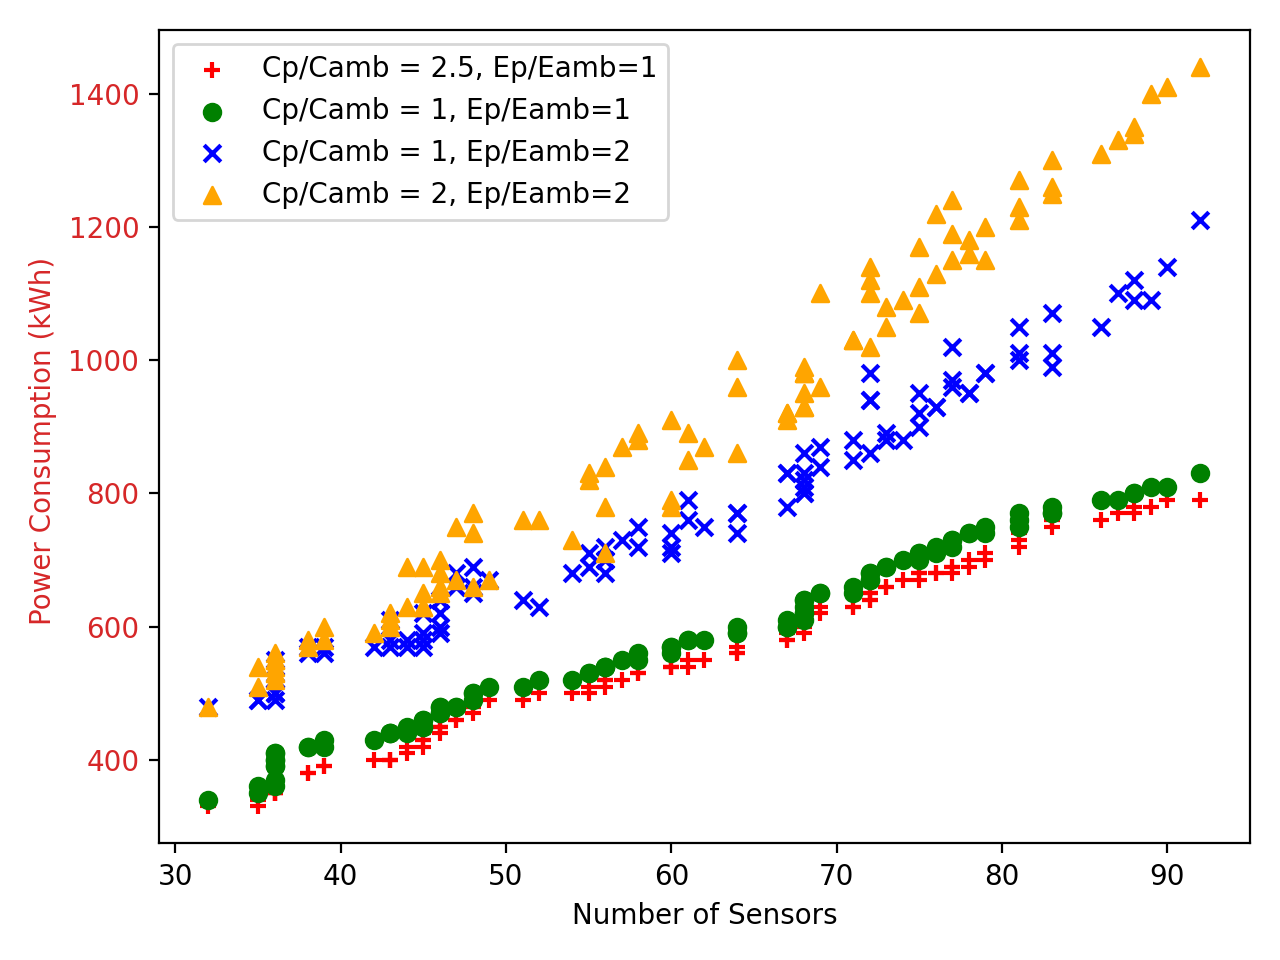
\includegraphics [width=0.47\textwidth] {img/powerVar.png} }\label{fig:powerVar}}%
    \caption{Evaluation of last generation chromosomes on capital cost $O_{cost}$  and operating energy footprint $O_{energy}$ .}
    \label{fig:businesstradeoffs}%
\end{figure}


The system is able to pick up sensors to achieve a Virtual Sensor Field configuration under all 4 experimental conditions with a forward translation  (MSE $\leq$ 0.2) . 
Figure \ref{fig:fwdbkwdVar} shows the distribution of $\{ O^v_f, O^v_b \}$ for the optimised last generation gene pool where number of sensors vary from $[30,96]$ and $\{ O^v_f, O^v_b \}$ lies between $\{ 0.02,1 \}$.
We see a natural affinity of the system to optimize the sensor field with minimal or less expensive sensor solution is evident from design spaces with high levels of backward MSE ($> 0.6$).
The capital and operating cost of the smart building solution is approximated in Figure \ref{fig:businesstradeoffs}.
We regress the best possible linear fit to approximate the rate of change of $O_{energy}, O_{cost}$ per additional sensor and fill up the entries of Tables \ref{table:powerMatrix} with the fitted slope.
% The slope of a line will indicate average change in metric for  intuitive key performance indicators on the system. 
% represent the change of power and capital required per additional sensor on average within the solution set. 
 

\begin{table}[]
\begin{tabular}{|l|l|l|}
\hline
     Market Segment  & Monthly Energy (kWh) & Capital $\$$      \\ \hline
 Home &  15 & 22.5 \\ \hline
 Community & 11 & 26.6 \\ \hline
 Co-Working & 8.8 & 24.5 \\ \hline
 Commercial  & 6.9  & 48.5  \\ \hline
\end{tabular}
\caption{Average Capital Cost and Monthly Energy Footprint for 4 different market segments   }
\label{table:powerMatrix}
\end{table}

% \begin{table}[]
% \begin{tabular}{|l|l|l|}
% \hline
%         $\$$/sensor & Ambient Sensor    & Power Meters       \\ \hline
% Do It Yourself  & Home $\approx$ 22.5  & Community   $\approx$  26.6    \\ \hline
% Industrial    & Co-Working   $\approx$  24.5   & Commercial    $\approx$  48.8 \\ \hline
% \end{tabular}
% \caption{Capital Required as per Market Segmentation for a 2 x 2 Ambient Sensing Solution Study }
% \label{table:capexMatrix}
% \end{table}
